\section{Local screening and electron counts}\label{sec:screening}\label{m:sec:screening}\label{a:sec:screening}

We now compare the quantum state in a ball with an unconstrained
Thomas--Fermi minimizer in the same ball.  The comparison has two outputs:
a uniform second-moment bound for the number of nearby electrons, and a
quantitative Coulomb-distance estimate for a finer local density.  Both
estimates hold for every $\delta$-state.  This stability under a small
increase of energy will be essential when we later condition on observations.
Throughout this section, $\psi$ is a normalized $\delta$-state in any finite
sector $n$: $q_n[\psi]\le E+\delta$, where
$E=\inf_k E_k$.  No eigenstate assumption or bound on $n$ is used here.
Expectations refer to its position and spin law, together with any
localization labels that are specified.

\subsection{Two local geometries}

Fix $A=40$.  We use either of the following scale geometries; the
choice is kept fixed throughout each application of this section.
All balls in these definitions are open.
\begin{equation}\label{m:eq:screen-scale}
 \begin{aligned}
 &\text{nuclear scale:}\qquad L=10^6,\quad\mathcal Y=\R^3,\\
 &\hspace{2em}a_y=\sup\{s>0:\nu(B(y,Ls))\le s^{-3}\};\\[.4ex]
 &\text{atomic distance scale:}\qquad L=10^5,\quad
 \nu=Z\delta_0,\\
 &\hspace{2em}\mathcal Y=\R^3\setminus\{0\},\qquad a_y=|y|/L.
 \end{aligned}
\end{equation}
Put $B_y=B(y,a_y)$ and $d_y=\min_m|y-R_m|$; in the atomic
geometry $d_y=|y|$.  The nuclear scale is used for molecular
estimates, including balls containing nuclei.  The atomic distance
scale gives nucleus-free patches at every positive distance from the
origin, also below $Z^{-1/3}$.  These scales are distinct: for a single
nucleus the first is $\max(Z^{-1/3},|y|/10^6)$.

\begin{lemma}[Properties of the nuclear scale]\label{m:lem:screen-scale}
In the nuclear-scale geometry, $a:\R^3\to(0,\infty)$ is
$L^{-1}$-Lipschitz and satisfies
\begin{equation}\label{m:eq:screen-scale-properties}
 Z^{-1/3}\le a_y<\infty,\quad
 \nu(B(y,La_y))\le a_y^{-3},\quad
 \nu(B(y,2La_y))>(2a_y)^{-3},\quad d_y\le La_y.
\end{equation}
If $d_y/L>1$, then $a_y=d_y/L$.  For every fixed $c<L/2$,
$B(y,ca_y)$ is covered by a bounded number of balls $B_z$ with
$a_z\asymp a_y$.  The covering bound depends only on $c$ and $L$.
\end{lemma}

\begin{proof}
The set of admissible $s$ in \eqref{m:eq:screen-scale} is downward closed.
It contains $Z^{-1/3}$ and is bounded above, since every sufficiently large
ball contains all nuclei.  Increasing open balls show that the condition
also holds at the supremum.  The radius $2a_y$ is not admissible, proving
the third inequality in \eqref{m:eq:screen-scale-properties}.

If $s=a_x-|x-y|/L>0$, then
$B(y,Ls)\subset B(x,La_x)$, and hence
$\nu(B(y,Ls))\le a_x^{-3}\le s^{-3}$.  Thus $a_y\ge s$.
Interchanging $x$ and $y$ proves the Lipschitz bound.  If $d_y>La_y$,
a slightly larger ball in the defining family would still contain no
nucleus, a contradiction.  If $d_y/L>1$, every radius below $d_y/L$ is
admissible, whereas every strictly larger radius contains a charge at
least one and has $s^{-3}<1$.  This proves the asserted equality.
Finally, the Lipschitz bound makes all scales in $B(y,ca_y)$ comparable
to $a_y$; a mesh of spacing a sufficiently small multiple of $a_y$
gives the stated cover.
\end{proof}

In the atomic geometry the scale is also $L^{-1}$-Lipschitz, and
$B(y,La_y)$ contains no nucleus.  Thus in both geometries
\[
 \nu(B(y,La_y))\le a_y^{-3}.
\]
For every fixed $c<L/2$, the ball $B(y,ca_y)$ stays in the target
domain $\mathcal Y$ and has a bounded cover by cells $B_z$ of scales
comparable to $a_y$.  In the atomic case this follows from
$|y|=La_y$ and the same mesh argument.  The proofs below use these
common local properties.  The lower scale bound $a_y\ge Z^{-1/3}$
is not assumed in the atomic case.

For the present $\delta$-state define
\begin{equation}\label{m:eq:screen-count-normalization}
 \begin{gathered}
 n_y=\#\{i:x_i\in B_y\},\qquad
 m_{0,y}=\max(a_y^{-3},1),\qquad
 m_y=m_{0,y}+\sqrt{\delta a_y},\qquad e_y=\frac{m_y^2}{a_y},\\
 P=\max\left(1,\sup_{y\in\mathcal Y}\frac{\E n_y^2}{m_y^2}\right).
 \end{gathered}
\end{equation}
Initially $P$ is merely finite, since $n_y\le n$ and $m_y\ge1$.
We shall prove that it is bounded by a universal constant.  Notice that
\begin{equation}\label{m:eq:screen-normalization-inequalities}
 m_y\ge1,\qquad a_y m_y\ge1,\qquad a_y m_y^{2/3}\ge1,
 \qquad e_y\asymp\max(a_y^{-7},a_y^{-1},\delta).
\end{equation}
These facts hold also when $a_y>1$.
Define the raw far field
\begin{equation}\label{m:eq:screen-raw-field}
 J_y=\int_{|v-y|\ge Aa_y}\frac{d\nu(v)}{|y-v|}
       -\sum_{|x_i-y|\ge Aa_y}\frac1{|y-x_i|}.
\end{equation}
The exclusion removes its singularities and, for each fixed system,
$|J_y|\le (Z+n)/(Aa_y)$.  In the atomic geometry the nuclear
term is exactly $V(y)=Z/|y|$, since $A<L$.

\subsection{A positive-field estimate}

A deterministic cut and its recorded out data $X$ have the meaning of
Lemma~\ref{lem:loc-identity}.  The next estimate permits a finite initial sequence of cuts;
the proof appends further deterministic cuts only to rule out a large
positive field.

\begin{lemma}[Conditional positive fields]\label{m:lem:screen-positive-field}\label{a:lem:screen-provisional}
Fix $C_0\ge1$. Suppose the initial sequence is absent, or its total out support is covered by at
most $C_0$ balls $B_z$ and the sum of its cuts' squared gradients is bounded by
\[
 \sum_z D_z^2a_z^{-2}\1_{B_z},
 \qquad \frac{D_z^2}{a_zm_z}\le C_0\sqrt P.
\]
If $X$ denotes its data (trivial for an absent sequence), and $e_*$ is the
maximum of $e_y$ and the energies $e_z$ of these covering cells, then
\begin{equation}\label{m:eq:screen-positive}
 \big\|(\E[J_y\mid X])_+\big\|_2
       \le C(C_0)\sqrt{\frac{P e_*}{a_y}}.
\end{equation}
\end{lemma}

\begin{proof}
We first give the upper trial at a target $y$.  Append a cut that is
full out on $B(y,Aa_y)$, supported in $B(y,2Aa_y)$, and has gradients
bounded by $C/a_y$.  Write $X'$ for the enlarged data, $a=a_y$, and
$h=\E[J_y\mid X']$.  The sliced core vanishes on $B(y,Aa)$.
Take uniform packet centers of total mass $M_{\rm tr}\ge0$ in $B(y,a)$, with
packet width $a$.  The packet support lies in $B(y,2a)$ and is separated
from the core.  The radial mean of the core field and of each far nuclear
field is its value at $y$.  Near nuclei contribute positively, and
$J_y$ subtracts far out electrons as well as the core.  Therefore
Lemma~\ref{lem:loc-hole-trial} gives
\begin{equation}\label{m:eq:screen-field-trial}
 E\le e_{X'}-M_{\rm tr}h+C\left(\frac{M_{\rm tr}^{5/3}}{a^2}
                     +\frac{M_{\rm tr}}{a^2}+\frac{M_{\rm tr}^2}{a}\right).
\end{equation}
Here $M_{\rm tr}$ is the expected occupation of the packet trial; it need not be
an integer.  This use of an arbitrary trial mass is justified by
$E=\inf_k E_k$.

For $ah>C_1m_{0,y}$ choose $M_{\rm tr}=\lambda ah$.  The three positive terms in
\eqref{m:eq:screen-field-trial}, divided by $M_{\rm tr}h$, are at most
\[
 \frac{C\lambda^{2/3}}{a(ah)^{1/3}},\qquad
 \frac{C}{a(ah)},\qquad C\lambda.
\]
The inequalities $am_{0,y}^{1/3}\ge1$ and $am_{0,y}\ge1$ allow us to
choose $\lambda>0$ small and then $C_1$ large so that their sum is less
than a fixed number below one.  In the other case use the vacuum trial.
For all data this proves
\begin{equation}\label{m:eq:screen-field-upper}
 E\le e_{X'}-ca h_+^2+C\frac{m_{0,y}^2}{a}.
\end{equation}

The insertion estimate makes a large positive field expensive.  We
bound the energy of the removed electrons in terms of positive fields
at nearby centers.  If the present field exceeded a universal multiple
of its proposed bound, this comparison would force a larger normalized
field after one further deterministic cut.  Repetition gives doubly
exponential growth, whereas the elementary nuclear bound and the
Lipschitz scale permit only exponential growth.  We now quantify this
argument, retaining the original $e_*$ throughout.

Start with target $v_0=y$ and the given data $X_0=X$.  At stage $j$,
append the cut just constructed at the current deterministic target
$v_j$; denote the enlarged data by $X_{j+1}$.  The upper estimate
\eqref{m:eq:screen-field-upper} applies with $y=v_j$ and
$X'=X_{j+1}$.  Cover the supports of all cuts, including this new cut,
by at most $C(j+1)$ local cells, and let $\mathcal U_j$ be the union
of their doubled balls $2B_z$.  These are the possible next targets:
we estimate the removed energy using their fields under the enlarged
data, writing $X'=X_{j+1}$ in this calculation.
Each newly added scale is comparable to a preceding covering scale
by the common local scale properties above; the original target and
initial covering scales need not be comparable to one another.
Let $a_{\min}>0$ be the minimum scale of the original target and
initial covering cells.  The Lipschitz property and the bounded local
meshes give, for every later target or covering cell at iteration $j$,
\begin{equation}\label{a:eq:screen-chain-units}
 a_v\ge C^{-(j+1)}a_{\min},\qquad e_v\le C^{j+1}e_*.
\end{equation}
Indeed each new scale is comparable to a preceding scale; the
quantities $m(a)=\max(a^{-3},1)+\sqrt{\delta a}$ and
$e(a)=m(a)^2/a$ change by a bounded factor when $a$ does, uniformly
in $\delta$.  The total out count obeys
\begin{equation}\label{a:eq:screen-chain-count}
 \|n_o\|_2\le\sum_{\text{covering cells }z}\|n_z\|_2
                  \le\sqrt P\sum_zm_z.
\end{equation}
The localization error is at most $C^{j+1}Pe_*$:
for an initial cell this follows from
\[
 D_z^2a_z^{-2}\E n_z
 \le\sqrt P\,\frac{D_z^2}{a_zm_z}e_z\le C_0Pe_z,
\]
and for a later cell it follows from
$a_zm_z\ge1$ and $\E n_z\le\sqrt Pm_z$.

For a covering cell $B_z$, let $V_z$ be the potential of nuclei in
$B(z,4a_z)$.  Let $h_z(v)$ be the conditional raw signed field, given
the present $X'$, of all sources at distance at least $4a_z$ from $z$.
It has a jointly measurable harmonic version on $3B_z$: all
sources are separated from compact subballs, so their kernel
derivatives are bounded for the fixed system and may be integrated
against the conditional law.  On $B_z$ the field of the conditional core
satisfies
\begin{equation}\label{m:eq:screen-field-decomposition}
 \Phi_{X'}\le V_z+h_z+\text{the far out-electron potential}.
\end{equation}
For $v\in2B_z$, the exclusion in $J_v$ contains $B(z,4a_z)$, since
$A=40$ and nearby scales are comparable.  Extra electrons in $h_z$
can only lower the field.  Extra nuclei have total charge at most
$a_z^{-3}$ and distance at least $2a_z$ from $v$.  Hence
\begin{equation}\label{m:eq:screen-harmonic-raw}
 h_z(v)\le\E[J_v\mid X']+Ca_z^{-4}.
\end{equation}
Set
\[
 G(v,X')=\sqrt{\frac{a_v}{e_*}}
           \big\|(\E[J_v\mid X'])_+\big\|_2.
\]
Positive parts of harmonic functions are subharmonic.  Their ball
submean inequality, a fixed covering of $B_z$, and Minkowski's inequality
give
\begin{align}\label{m:eq:screen-harmonic-sup}
 \left\|\sup_{B_z}(h_z)_+\right\|_2
 &\le Ca_z^{-3}\int_{2B_z}\|(h_z(v))_+\|_2\,dv\\
 &\le C^{j+1}\sqrt{\frac{e_*}{a_z}}
        \left(1+\sup_vG(v,X')\right),\notag
\end{align}
where the supremum is over $v\in\mathcal U_j$.  The term
$a_z^{-4}$ was absorbed using $a_z^{-7}\le e_z\le C^{j+1}e_*$.

The out addback in \eqref{m:eq:screen-field-decomposition} is at most
\[
 C\sum_l\frac{n_l}{\max(a_l,a_z)}.
\]
Indeed the far exclusion gives distance at least $3a_z$; if
$a_l\gg a_z$, Lipschitzness of the scale forces every point of $B_l$
to be a distance at least a fixed multiple of $a_l$ from $B_z$.
Using $\|n_l\|_2\le\sqrt{Pe_la_l}$ and
$\sqrt{a_l}/\max(a_l,a_z)\le a_z^{-1/2}$ bounds this addback in
$L^2$ by $C^{j+1}\sqrt{Pe_*/a_z}$.

For completeness, the nuclear singularities have the required energy
scale.  If $Q_z=\nu(B(z,4a_z))\le a_z^{-3}$, weighted convexity gives
\begin{equation}\label{m:eq:screen-nuclear-power}
 \int_{B_z}V_z^{5/2}
 \le Q_z^{3/2}\sum_m z_m
       \int_{B_z}|v-R_m|^{-5/2}\,dv
 \le C Q_z^{5/2}a_z^{1/2}\le Ca_z^{-7}.
\end{equation}
In the sum over cells, the power of the number of cells arising from
convexity is bounded by $C^{j+1}$.  Lemma~\ref{lem:loc-kinetic} and
Young's inequality therefore absorb this attraction at cost
$C^{j+1}e_*$.  Multiplying the other bounds by
$\|n_z\|_2\le\sqrt{Pe_za_z}$ and summing cells, the conditional
localization identity, with out-pair repulsion dropped, yields
\begin{equation}\label{m:eq:screen-field-lower}
 q_n[\psi]+\mathrm{IMS}
 \ge\E e_{X'}-C^{j+1}e_*
           \left(P+\sqrt P\sup_vG(v,X')\right).
\end{equation}
This calculation used the actual list of cuts; it did not assume the
conclusion of the lemma for that list.

Combine \eqref{m:eq:screen-field-upper} and
\eqref{m:eq:screen-field-lower}, use $\delta\le e_*$, and apply conditional
Jensen from the enlarged data back to the preceding data.  With
$G(v_j,X_j)$ defined by the same normalization,
\begin{equation}\label{a:eq:screen-recursion}
 G(v_j,X_j)^2\le C^{j+1}
       \left(P+\sqrt P\sup_{v\in\mathcal U_j}G(v,X_{j+1})\right).
\end{equation}
Write $g_j=G(v_j,X_j)/\sqrt P$.  Whenever $g_j^2\ge2C^{j+1}$,
the last inequality permits a deterministic next target
$v_{j+1}\in\mathcal U_j$ with
\[
 g_{j+1}\ge\frac{g_j^2}{4C^{j+1}},\qquad
 \log g_{j+1}\ge2\log g_j-(j+1)\log C-\log4.
\]
The series
\[
 S=\sum_{j\ge0}2^{-j-1}\big((j+1)\log C+\log4\big)
\]
converges.  Choose $M_0>0$ so that
$\exp(2^{j+1}M_0)\ge2C^{j+1}$ for every $j$.  If
$\log g_0>S+M_0$, induction gives $\log g_j\ge2^jM_0$;
thus the condition for selecting each next target always holds.
All supremums here are of numerical norms for deterministic cuts;
choosing a target close to one of them never chooses a target from
sampled data.  On the other hand, $J_v\le Z/(Aa_v)$ pointwise, and
\eqref{a:eq:screen-chain-units} gives
\[
 G(v,X')\le\sqrt{\frac{a_v}{e_*}}\frac{Z}{Aa_v}
 \le C^{j+1}\frac{Z}{A\sqrt{e_*a_{\min}}}.
\]
For the fixed system and initial cuts the last factor is finite.
Its logarithm grows at most linearly in $j$, contradicting the
positive multiple of $2^j$ forced above.  This argument works in
both geometries and requires no global lower bound on the scale.
It proves \eqref{m:eq:screen-positive}.
\end{proof}

\subsection{Comparison in a ball}

We now use the positive-field estimate to control the full local
quantum energy.  Besides bounding counts, the comparison retains its
Coulomb error and the cost of placing electrons where the comparison
field is negative.  We use the constants
\[
 p=\frac32,\qquad k=\left(\frac53\cT\right)^{-3/2},\qquad \cF=4\pi k.
\]

\begin{lemma}[Conditional comparison in an interior ball]\label{m:lem:screen-patch}\label{a:lem:screen-patch}
Fix $y\in\mathcal Y$, write $a=a_y$, $m=m_y$, $e=e_y$, and choose
$0<\beta<1/100$ such that
\begin{equation}\label{m:eq:screen-patch-condition}
 \frac{\beta^{-2}}{am}\le\sqrt P.
\end{equation}
Set $b=\beta a$.  There is a deterministic $t_0\in[5a,6a]$ and a cut full out on
$B(y,t_0)$, supported in $B(y,t_0+b)$, with gradients at most $C/b$.
Let $X$ be its out data, $\rho_X^c$ the conditional core density,
$\Phi_X=V-K*\rho_X^c$, and $\Omega=B(y,t_0-4b)$.
There is a unique minimizer $\rho=\rho_X\ge0$, extended by zero
outside $\Omega$, of
\begin{equation}\label{m:eq:screen-tf-functional}
 \mathcal T_X(\rho)=\cT\int\rho^{5/3}-\int\Phi_X\rho+D(\rho).
\end{equation}
It is measurable in $X$ and, with $W=\Phi_X-K*\rho$, satisfies
\begin{equation}\label{m:eq:screen-tf-equation}
 \rho=kW_+^{3/2}\quad\hbox{in }\Omega.
\end{equation}
Retain the out particles with $|x_i-y|<t_0-7b$ and put
$\sigma=\sum_{i\ \mathrm{retained}}\vartheta_b(\cdot-x_i)$, using the
radial fine kernel from Lemma~\ref{lem:loc-cubes}.  Write
\begin{equation}\label{m:eq:screen-remainder}
 \mathcal L=\cT\int\left(\sigma^{5/3}-\rho^{5/3}
              -\frac53\rho^{2/3}(\sigma-\rho)\right).
\end{equation}
For every sufficiently small $\epsilon>0$,
\begin{align}\label{m:eq:screen-comparison}
 &\E\left[D(\sigma-\rho)+\mathcal L+\int W_-\sigma\right]\\
 &\quad\le C\left[\delta+(\epsilon+\sqrt\beta)Pe
       +\epsilon^{-3/2}\beta^{1/2}a^{-7}
       +b^{-1}\sqrt Pm
       +b^{-2}\left(P^{2/3}m^{4/3}+\sqrt Pm\right)\right].\notag
\end{align}
Moreover, $\E\int\sigma^{5/3}$ is bounded by $CPe$ plus a constant
times this right-hand side, and the out kinetic energy obeys
\begin{equation}\label{m:eq:screen-out-kinetic}
 T_o\le C\left(Pe+b^{-2}\sqrt Pm\right).
\end{equation}
Finally, independently of the data,
\begin{equation}\label{m:eq:screen-interior-upper}
 W\le V_{\rm loc}+Ca^{-4}\quad\hbox{on }B(y,3a),\qquad
 \int_{B(y,2a)}\rho\le Ca^{-3},
\end{equation}
where $V_{\rm loc}$ is the potential of nuclei in $B(y,20a)$.
If this local nuclear measure is zero, as it always is in the atomic
distance geometry, the same construction has the sharper bound
\begin{equation}\label{a:eq:screen-patch}
 \E\left[D(\sigma-\rho)+\mathcal L+\int W_-\sigma\right]
 \le C\left[\delta+\sqrt\beta Pe+b^{-1}\sqrt Pm
       +b^{-2}\left(P^{2/3}m^{4/3}+\sqrt Pm\right)\right],
\end{equation}
and its interior bounds include
\begin{equation}\label{a:eq:screen-interior}
 W\le Ca^{-4},\qquad \rho\le Ca^{-6}
       \quad\hbox{on }B(y,3a),\qquad
 \int_{B(y,2a)}\rho\le Ca^{-3}.
\end{equation}
\end{lemma}

The Coulomb error $D(\sigma-\rho)$ controls smooth tests of
$\sigma-\rho$ in mean, leaving exceptional cut data possible.  The
penalty $\int W_-\sigma$ integrates the negative field against the
fine density of retained electrons.
Together with the later oscillation estimates and a lower bound on
this density's local mass, it provides the additional control needed
to pass a lower field estimate to expectation.

\begin{proof}
We divide the proof into the choice of cut, the two energy comparisons,
and the deterministic interior bound.


\begin{figure}[htbp]
 \centering
 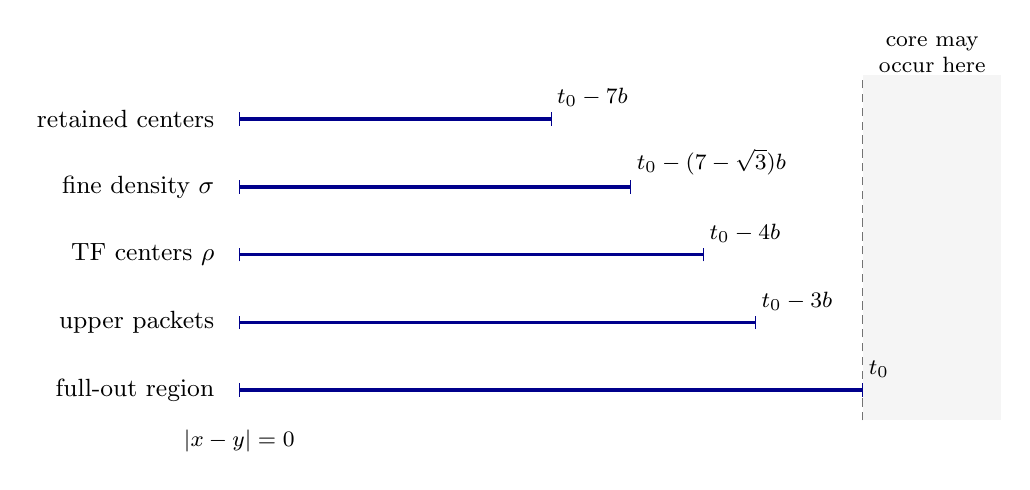
\begin{tikzpicture}[x=.88cm,y=.86cm,font=\small]
  \fill[black!4] (9,-.45) rectangle (11,4.65);
  \draw[densely dashed,black!55] (9,-.45)--(9,4.65);
  \node[align=center,font=\footnotesize] at (10,4.95) {core may\\occur here};
  \foreach \yy/\endx/\lefttext/\righttext in {
       4/4.5/{retained centers}/{$t_0-7b$},
       3/5.65/{fine density $\sigma$}/{$t_0-(7-\sqrt3)b$},
       2/6.7/{TF centers $\rho$}/{$t_0-4b$},
       1/7.45/{upper packets}/{$t_0-3b$},
       0/9/{full-out region}/{$t_0$}} {
    \node[anchor=east] at (-.22,\yy) {\lefttext};
    \draw[very thick,blue!55!black] (0,\yy)--(\endx,\yy);
    \draw[blue!55!black] (0,\yy-.1)--(0,\yy+.1);
    \draw[blue!55!black] (\endx,\yy-.1)--(\endx,\yy+.1);
    \node[anchor=south west,font=\footnotesize,inner sep=2pt]
      at (\endx,\yy+.09) {\righttext};
  }
  \node[anchor=north,font=\footnotesize] at (0,-.45) {$|x-y|=0$};
\end{tikzpicture}

 \caption{Radial supports in the interior comparison (schematic, not to
 scale). Fine smears of retained particles lie inside the TF domain,
 and the upper packets remain at distance at least $3b$ from the
 conditional core. This particle-support geometry is common to both
 applications. The atomic distance scale makes $B(y,20a)$ free of
 nuclei; the molecular scale may leave nuclei there, and their packet
 loss is retained in \eqref{m:eq:screen-comparison}.}
 \label{m:fig:screen-patch}
\end{figure}

\paragraph{Choice of cut and the conditional field.}
For a candidate $t\in[5a,6a]$, let the cut transition in a shell of
width $b$, using sine and cosine of an angle.  Let $n_{\rm del}$ count
the out particles not retained.  Such a particle lies in
$t-7b\le|x-y|\le t+b$.  For each raw pair of particles the set of
$t$ for which both lie in this shell has length at most $8b$.
Averaging over $t$ therefore bounds its expected squared count by
$C\beta Pm^2$, since $B(y,7a)$ has a bounded comparable-scale cover.
The same averaging, applied to the nuclear integral, uses
\eqref{m:eq:screen-nuclear-power} to give a bound $C\beta a^{-7}$.
Averaging the sum of the two normalized nonnegative quantities selects
one $t_0$ for which both bounds hold:
\begin{equation}\label{m:eq:screen-deleted-shell}
 \begin{gathered}
 \E n_{\rm del}^2\le C\beta Pm^2,\qquad
 \E n_o^2\le CPm^2,\qquad
 \mathrm{IMS}\le Cb^{-2}\sqrt Pm,\\
 \int_{\{t_0-7b\le|x-y|\le t_0+b\}}V_{\rm loc}^{5/2}
       \le C\beta a^{-7}.
 \end{gathered}
\end{equation}
The full out-count and IMS bounds in the same display follow from
the comparable-scale cover and $\E n_z\le\sqrt Pm_z$.

On the cut support and on $\Omega$ we have
\begin{equation}\label{m:eq:screen-field-cap}
 \Phi_X\le V_{\rm loc}+F,\qquad F\ge0,\qquad
 \|F\|_2\le C\frac{\sqrt Pm}{a}.
\end{equation}
To see this, the raw sources outside $B(y,20a)$ give a harmonic
conditional field on $B(y,10a)$; these electrons are all core particles.
Its value at $v\in B(y,10a)$ is at most
$\E[J_v\mid X]+Ca^{-4}$, by the same exclusion comparison as
\eqref{m:eq:screen-harmonic-raw}.  Take $F$ to be the positive supremum
on $B(y,7a)$.  Harmonic means and
Lemma~\ref{m:lem:screen-positive-field} prove \eqref{m:eq:screen-field-cap}.
The cells of this initial cut have scale comparable to $a$ and
$D_z\le C\beta^{-1}$, so \eqref{m:eq:screen-patch-condition} verifies
that lemma's hypothesis.

\paragraph{The unconstrained minimizer.}
The core is at distance at least $4b$ from $\Omega$, so its potential
is bounded and smooth there.  Hence $\Phi_X\in L^{5/2}(\Omega)$.
Young's inequality makes \eqref{m:eq:screen-tf-functional} coercive in
$L^{5/3}$.  The positive Coulomb form is weakly lower semicontinuous:
by Lemma~\ref{lem:loc-coulomb} it is a squared Hilbert norm, or
one may express it as the supremum of its affine dual forms.
The direct method on the closed positive cone gives a minimizer,
and strict convexity of the kinetic term gives uniqueness.
Nonnegative variations, followed by signed compact multiplicative
variations, give
\[
 \frac53\cT\rho^{2/3}-\Phi_X+K*\rho\ge0,
 \qquad
 \left(\frac53\cT\rho^{2/3}-\Phi_X+K*\rho\right)\rho=0,
\]
which is \eqref{m:eq:screen-tf-equation}.

This minimizer depends continuously in $L^{5/3}$ on its field in
$L^{5/2}$.  Indeed convergent fields give uniformly bounded minimizers;
weak lower semicontinuity and comparison with the limit minimizer
identify each weak limit and give convergence of the minimum values.
Lower semicontinuity of $D$ then forces convergence of the kinetic
norms.  Uniform convexity of $L^{5/3}$ gives strong convergence.
The conditional field, being jointly measurable and taking values
in the separable space $L^{5/2}(\Omega)$, is measurable as a
function with values in that space.  The continuity just proved
establishes the stated measurability of $\rho$.

The diameter of $\Omega$ is at most $12a$, so
$D(\rho)\ge(\int\rho)^2/(24a)$.  The minimum is nonpositive because
zero is admissible.  Absorbing $V_{\rm loc}$ with Young's inequality
in \eqref{m:eq:screen-field-cap} gives
\[
 \frac{(\int\rho)^2}{Ca}\le Ca^{-7}+F\int\rho.
\]
It follows that
\begin{equation}\label{m:eq:screen-tf-mass}
 \int\rho\le C(aF+a^{-3}),\qquad
 \int\rho^{5/3}\le C(aF^2+a^{-7}).
\end{equation}
When $V_{\rm loc}=0$, the same nonpositive-minimum argument uses
only $\Phi_X\le F$ and gives the sharper estimates
\begin{equation}\label{a:eq:screen-minimizer-mass}
 \int\rho\le CaF,\qquad \int\rho^{5/3}\le CaF^2.
\end{equation}
In particular all trial errors below are integrable in $X$.

\paragraph{Upper quantum comparison.}
The centers $\rho$ lie in $\Omega=B(y,t_0-4b)$; packets of width
$b$ remain at distance at least $3b$ from the core.  Thus
Lemma~\ref{lem:loc-hole-trial} applies, and radial smearing leaves
the core potential unchanged.  The nuclear loss is bounded at
centers by
\[
 V_b^{\rm loss}(x)=\sum_{R_m\in B(y,20a)}
             \frac{z_m}{|x-R_m|}\1_{\{|x-R_m|\le2b\}}.
\]
Weighted convexity, the total local charge bound, and integration of
$|x|^{-5/2}$ over a ball of radius $2b$ give
\[
 \int(V_b^{\rm loss})^{5/2}\le C\beta^{1/2}a^{-7}.
\]
Nuclei not in the indicated local ball are harmonic on all packets.
Young's inequality now gives, pathwise,
\begin{equation}\label{m:eq:screen-patch-upper}
 E\le e_X+\mathcal T_X(\rho)+Cb^{-2}\int\rho
       +C\epsilon\int\rho^{5/3}
       +C\epsilon^{-3/2}\beta^{1/2}a^{-7}.
\end{equation}

\paragraph{Lower quantum comparison.}
Reserve a fraction $\epsilon T_o$ of the out kinetic energy.  The
coarse kinetic inequality absorbs both $V_b^{\rm loss}$ and the
nuclear attraction of deleted particles, at cost
$C\epsilon^{-3/2}\beta^{1/2}a^{-7}$, using
\eqref{m:eq:screen-deleted-shell}.  The deleted $F$ contribution costs
at most
\[
 \|F\|_2\|n_{\rm del}\|_2\le C\sqrt\beta Pe.
\]
The retained fine density $\sigma$ is supported in $\Omega$, because
its centers have radius less than $t_0-7b$ and its kernel radius is
$\sqrt3b$.  The core potential is harmonic on these kernels, and
the loss of nuclear attraction is again covered by $V_b^{\rm loss}$
at the actual particle positions.  Applying the remaining fraction
of Lemma~\ref{lem:loc-cubes} and its pair-repulsion bound in the
localization identity gives
\begin{align}\label{m:eq:screen-patch-lower}
 q_n[\psi]+\mathrm{IMS}
 &\ge\E\left[e_X+\mathcal T_X(\sigma)
                    -\epsilon\cT\int\sigma^{5/3}\right]
       -C\mathcal R,\\
 \mathcal R&=\epsilon^{-3/2}\beta^{1/2}a^{-7}
             +\sqrt\beta Pe+b^{-1}\sqrt Pm
             +b^{-2}\left(P^{2/3}m^{4/3}+\sqrt Pm\right).\notag
\end{align}
Here $\E n_o^{4/3}\le(\E n_o^2)^{2/3}$; no higher out-count
moment is required.

The Euler equation gives the exact expansion
\begin{equation}\label{m:eq:screen-tf-expansion}
 \mathcal T_X(\sigma)-\mathcal T_X(\rho)
       =D(\sigma-\rho)+\mathcal L+\int W_-\sigma.
\end{equation}
Besides being nonnegative, the convex remainder satisfies
\[
 \mathcal L\ge c\int\sigma^{5/3}-C\int\rho^{5/3},
\]
by Young's inequality applied to the tangent term.  For small
$\epsilon$ this absorbs $\epsilon\cT\int\sigma^{5/3}$ into half
of $\mathcal L$, with error $C\epsilon\int\rho^{5/3}$.
Average \eqref{m:eq:screen-patch-upper}, compare it with
\eqref{m:eq:screen-patch-lower}, and use
\eqref{m:eq:screen-tf-mass}, \eqref{m:eq:screen-field-cap}, and the IMS
bound.  The terms $\epsilon\E\int\rho^{5/3}$ cost $C\epsilon Pe$;
the packet kinetic term costs
$Cb^{-2}(\sqrt Pm+a^{-3})\le Cb^{-2}\sqrt Pm$.
This proves \eqref{m:eq:screen-comparison}, after multiplying its
constant to restore the full nonnegative remainder, and also the
asserted bound for $\E\int\sigma^{5/3}$.

\paragraph{The source-free improvement.}
If $\nu(B(y,20a))=0$, every nucleus and the conditional core are
outside the packet supports.  The field $\Phi_X$ is harmonic on
those supports, so radial averaging is exact and the upper comparison
is
\begin{equation}\label{a:eq:screen-upper}
 E\le e_X+\mathcal T_X(\rho)+Cb^{-2}\int\rho.
\end{equation}
For the lower comparison, use all the out kinetic energy.
Harmonicity and the deleted-count bound give
\[
 \sum_{i\ \mathrm{retained}}\Phi_X(x_i)=\int\Phi_X\sigma,
 \qquad \E(Fn_{\rm del})\le C\sqrt\beta Pe.
\]
The full sharp kinetic
and pair bounds of Lemma~\ref{lem:loc-cubes} therefore give
\begin{equation}\label{a:eq:screen-lower}
 q_n[\psi]+\mathrm{IMS}
 \ge\E[e_X+\mathcal T_X(\sigma)]
 -C\left[\sqrt\beta Pe+b^{-1}\sqrt Pm
       +b^{-2}(P^{2/3}m^{4/3}+\sqrt Pm)\right].
\end{equation}
Subtract the average upper inequality and use the exact expansion
\eqref{m:eq:screen-tf-expansion}, the mass estimate
\eqref{a:eq:screen-minimizer-mass}, and the IMS bound.  This proves
\eqref{a:eq:screen-patch}, including its full convex remainder,
without the nuclear loss or an $\epsilon$ error.

There is a useful separate kinetic bound.  In the localization identity
use only $e_X\ge E$, drop pair repulsion, and use
\eqref{m:eq:screen-field-cap}.  Half the coarse kinetic inequality
absorbs $V_{\rm loc}$ at cost $Ca^{-7}$; also
$\E(Fn_o)\le CPe$.  The result is
\eqref{m:eq:screen-out-kinetic}.

\paragraph{Interior field bound.}
The core vanishes in $B(y,4a)$ and this ball lies in $\Omega$.
There
\[
 \Delta W=-4\pi\nu+\cF W_+^{3/2}.
\]
Put $s=4a$ and
\[
 U(x)=V_{\rm loc}(x)+\frac{C s^4}{(s^2-|x-y|^2)^4}.
\]
The Laplacian of the bump is at most
$80Cs^6/(s^2-|x-y|^2)^6$.  For a sufficiently large universal $C$
this is at most $\cF$ times its $3/2$ power.  Thus $U$ is a
supersolution for the displayed equation.  The difference $W-V_{\rm loc}$
is bounded above: the far nuclear field is bounded on this ball,
the core potential is nonnegative, and $K*\rho\ge0$.
Consequently $(W-U)_+$ has compact support inside the ball.
Nuclear singularities cancel in $W-U$, which is locally $H^1$;
testing the difference inequality by its positive part yields
\[
 -\int|\nabla(W-U)_+|^2
 \ge\cF\int_{\{W>U\}}(W_+^{3/2}-U^{3/2})(W-U)\ge0.
\]
The test is valid by compact $H^1$ approximation: the densities
are locally in $L^{5/3}$, and the nuclear point terms have already
canceled.  Hence $W\le U$.  On $B(y,3a)$ the bump is $Ca^{-4}$,
proving the first part of \eqref{m:eq:screen-interior-upper}.
If $V_{\rm loc}=0$, this yields $W\le Ca^{-4}$; the Euler equation
then gives $\rho\le Ca^{-6}$ and proves
\eqref{a:eq:screen-interior}.  In this source-free case,
\begin{equation}\label{a:eq:screen-poisson}
 \Delta W=\cF W_+^{3/2}=4\pi\rho
       \quad\hbox{on }B(y,4a).
\end{equation}
Finally, weighted powers and $\nu(B(y,20a))\le a^{-3}$ give
\[
 \int_{B(y,2a)}\rho
 \le C\int_{B(y,2a)}(V_{\rm loc}^{3/2}+a^{-6})
 \le C(a^{-9/2}a^{3/2}+a^{-3})\le Ca^{-3}.
\]
\end{proof}

\subsection{Closing the count estimate}

The comparison in a hole bounds its electron count through a smooth
Coulomb test.  The resulting inequality improves any sufficiently
large value of the provisional constant $P$, and therefore makes
that constant universal.

\begin{lemma}[Local second moments]\label{m:lem:screen-count}
For every normalized $\delta$-state in any finite sector and every
$y\in\mathcal Y$,
\begin{equation}\label{m:eq:screen-count}
 \E n_y^2\le C\left(\max(a_y^{-6},1)+\delta a_y\right).
\end{equation}
In particular the number $P$ in
\eqref{m:eq:screen-count-normalization} is at most a universal constant.
\end{lemma}

\begin{proof}
Fix small $\epsilon>0$ and $0<\beta<1/100$, to be chosen in that
order.  We need only consider $P\ge\beta^{-4}$, since $\beta$ will
be fixed universally.  Then $\beta^{-2}/(am)\le\sqrt P$ at every
target, and the patch of Lemma~\ref{m:lem:screen-patch} is available.
Every raw particle in $B_y$ is retained, and its fine smear is
contained in $B(y,1.1a)$ because $\beta<1/100$.
Choose a nonnegative smooth $\chi$, equal to one there, supported
in $B(y,2a)$, with $\|\nabla\chi\|_2\le C\sqrt a$.
Lemma~\ref{lem:loc-coulomb} and
\eqref{m:eq:screen-interior-upper} give
\[
 n_y\le\int\chi\sigma
 \le Ca^{-3}+C\sqrt{aD(\sigma-\rho)},\qquad
 \E n_y^2\le Ca^{-6}+Ca\,\E D(\sigma-\rho).
\]
Divide by $Pm^2$ and use \eqref{m:eq:screen-comparison}.  Since
$\delta a\le m^2$, the result is at most
\begin{align}\label{m:eq:screen-bootstrap-ratio}
 C\bigg[&P^{-1}+\epsilon+\sqrt\beta
       +\frac{\epsilon^{-3/2}\beta^{1/2}}P
       +\frac{\beta^{-1}}{\sqrt Pm}\\
       &+\frac{\beta^{-2}}{P^{1/3}am^{2/3}}
       +\frac{\beta^{-2}}{\sqrt Pam}\bigg].\notag
\end{align}
In the atomic distance geometry, using \eqref{a:eq:screen-patch}
instead gives the sharper intermediate inequality
\begin{equation}\label{a:eq:screen-count-bootstrap}
 \frac{\E n_y^2}{Pm_y^2}
 \le C\left[P^{-1}+\sqrt\beta
 +\frac{\beta^{-1}}{\sqrt Pm_y}
 +\frac{\beta^{-2}}{P^{1/3}a_ym_y^{2/3}}
 +\frac{\beta^{-2}}{\sqrt P a_ym_y}\right].
\end{equation}
For the common bound it suffices to use
\eqref{m:eq:screen-bootstrap-ratio} in both geometries.
First choose $\epsilon$ small, then $\beta$ small, and finally a
universal threshold $P_0$ large.  The inequalities
\eqref{m:eq:screen-normalization-inequalities} show that the expression
is at most $1/2$ whenever $P>P_0$.  Enlarge $P_0$ so that
$P_0\ge\beta^{-4}$; this verifies
\eqref{m:eq:screen-patch-condition} at every target.  If $P>P_0$, we
would obtain $\E n_y^2/m_y^2\le P/2$ for every $y$, contradicting
the definition of $P$.  Thus $P\le P_0$.  Since
$m_y^2\le2\max(a_y^{-6},1)+2\delta a_y$, this proves
\eqref{m:eq:screen-count}.
\end{proof}

\begin{proposition}[Uniform local counts and conditional fields]
\label{a:prop:screen-local}
In either geometry, every normalized $\delta$-state in a finite sector
satisfies $P\le C$.  Fix $y\in\mathcal Y$.  Suppose the initial
finite sequence of cuts has total out support covered by at most
$C_0$ cells $B_z$, with $C_0^{-1}\le a_z/a_y\le C_0$, and satisfies
the gradient hypothesis of Lemma~\ref{m:lem:screen-positive-field}.
The absent-cut case is allowed.  Then
\begin{equation}\label{a:eq:screen-local}
 P\le C,\qquad
 \big\|(\E[J_y\mid X])_+\big\|_2
             \le C(C_0)\frac{m_y}{a_y}.
\end{equation}
Neither constant depends on the nuclear system, particle number,
state, target, or $\delta$.
\end{proposition}

\begin{proof}
The count assertion is Lemma~\ref{m:lem:screen-count}.
Comparable scales have comparable $m$ and $e=m^2/a$, uniformly in
$\delta$, so $e_*\le C(C_0)e_y$ in
Lemma~\ref{m:lem:screen-positive-field}.  Substitute $P\le C$
into that lemma to obtain the field assertion.
\end{proof}

\begin{lemma}[Fine comparison and local density]\label{m:lem:screen-density}\label{a:cor:screen-refined}
There is a universal $a_0>0$ with the following property.  If
$a=a_y<a_0$ and $\psi$ is a $\delta$-state with
$\delta\le a^{-7+0.02}$, choose the patch of
Lemma~\ref{m:lem:screen-patch} with $b=a^{1+0.2}$.  Its densities obey
\begin{equation}\label{m:eq:screen-fine-error}
 \E\left[D(\sigma-\rho)+\mathcal L+\int W_-\sigma\right]
       \le Ca^{-7+0.02},\qquad
 \E\int\sigma^{5/3}\le Ca^{-7}.
\end{equation}
The raw one-body density satisfies
\begin{equation}\label{m:eq:screen-density}
 \int_{B(y,4a)}\rho_\psi^{5/3}\le Ca^{-7}.
\end{equation}
In particular, the two estimates needed in the atomic application are
\begin{equation}\label{a:eq:screen-refined}
 \E\left[D(\sigma-\rho)+\int W_-\sigma\right]\le Ca^{-7+.02},
 \qquad \int_{B(y,4a)}\rho_\psi^{5/3}\le Ca^{-7}.
\end{equation}
\end{lemma}

\begin{proof}
Take $\beta=a^{0.2}$ and $\epsilon=a^{0.02}$.  The energy assumption
gives $m\le Ca^{-3}$, while
$\beta^{-2}/(am)\le a^{1.6}$, so the patch hypothesis holds for
small $a$.  By Lemma~\ref{m:lem:screen-count}, $P\le C$.
The terms on the right of \eqref{m:eq:screen-comparison} are bounded
respectively by constant multiples of
\[
 a^{-6.98},\quad a^{-6.98}+a^{-6.9},\quad
 a^{-6.93},\quad a^{-4.2},\quad a^{-6.4}+a^{-5.4}.
\]
All are at most $Ca^{-7+0.02}$ for $a<1$, proving
\eqref{m:eq:screen-fine-error}.  Equation~\eqref{m:eq:screen-out-kinetic}
gives $T_o\le Ca^{-7}$.  Since the cut is full out on $B(y,4a)$,
the out density equals $\rho_\psi$ there.  Applying
Lemma~\ref{lem:loc-kinetic} proves \eqref{m:eq:screen-density}.
\end{proof}

\begin{corollary}[Raw near-Coulomb bound]
Under the hypotheses of Lemma~\ref{m:lem:screen-density}, for
$0<u\le4a$,
\begin{equation}\label{a:eq:screen-near-coulomb}
 \E\sum_{|x_i-y|<u}\frac1{|x_i-y|}
       \le Ca^{-4}(u/a)^{1/5}.
\end{equation}
\end{corollary}

\begin{proof}
The expectation is $\int_{B(y,u)}|x-y|^{-1}\rho_\psi(x)\,dx$.
H\"older's inequality, the raw density bound, and direct radial
integration give
\[
 \int_{B(y,u)}\frac{\rho_\psi(x)}{|x-y|}\,dx
 \le\left(\int_{B(y,4a)}\rho_\psi^{5/3}\right)^{3/5}
       \left(\int_{|z|<u}|z|^{-5/2}\,dz\right)^{2/5}
 \le Ca^{-21/5}u^{1/5}.
\]
This is the stated bound in either geometry.
\end{proof}

\subsection{Source-free oscillation and atomic annuli}

The next estimate controls also a very negative field.  It applies
when the patch contains no local nuclear source; molecular patches
containing nuclei instead use the offset oscillation estimate proved
with the nuclear splitting below.

\begin{lemma}[Interior oscillation]
\label{a:lem:screen-oscillation}
For every patch in Lemma~\ref{a:lem:screen-patch} with
$\nu(B(y,20a))=0$, and every
$0<s'\le a/2$, almost surely in its data,
\begin{equation}\label{a:eq:screen-oscillation}
 \sup_{x\in B(y,s')}|W(x)-W(y)|
       \le C\frac{s'}a\bigl(a^{-4}+W(y)_-\bigr).
\end{equation}
\end{lemma}

\begin{proof}
By \eqref{a:eq:screen-poisson} and \eqref{a:eq:screen-interior},
$0\le\Delta W\le Ca^{-6}$ on $B(y,2a)$.  Write
\[
 Q(x)=\frac1{4\pi}
       \int_{B(y,2a)}\frac{\Delta W(z)}{|x-z|}\,\dd z.
\]
For $x\in B(y,2a)$, direct integration of $|x-z|^{-1}$ and
$|x-z|^{-2}$ gives
\[
 0\le Q(x)\le Ca^{-4},\qquad |\nabla Q(x)|\le Ca^{-5}.
\]
Since $\Delta Q=-\Delta W$ inside that ball,
$H=W+Q$ is harmonic there.  By \eqref{a:eq:screen-interior},
$H\le C_1a^{-4}$.  Choose $C_2>C_1$ universally and put
$h=C_2a^{-4}-H$, a positive harmonic function on $B(y,2a)$.
The Poisson formula on a sphere of radius $3a/2$ gives
\[
 \sup_{B(y,a)}|\nabla h|\le Ca^{-1}h(y).
\]
Indeed the differentiated Poisson kernel on $B(y,a)$ is bounded
by $C/a$ times its value at the center; integrating the
nonnegative boundary values gives precisely this inequality.
Also $h(y)\le Ca^{-4}+W(y)_-$, since $Q(y)\ge0$.
Integrate the gradient along segments in $B(y,s')$, and add
the bound for $\nabla Q$.  This proves
\eqref{a:eq:screen-oscillation}.
\end{proof}

\begin{corollary}[Annular counts]
\label{a:cor:screen-annular}
In the atomic distance geometry, for every
$0<\lambda<\Lambda<\infty$ and $u>0$, every normalized
$\delta$-state of finite particle number satisfies
\begin{equation}\label{a:eq:screen-annular}
 \left\|\#\{i:\lambda u<|x_i|<\Lambda u\}\right\|_2
 \le C_{\lambda,\Lambda}
       \bigl(\max(u^{-3},1)+\sqrt{\delta u}\bigr).
\end{equation}
All constants are independent of $Z$ and of the particle number.
\end{corollary}

\begin{proof}
The compact annulus $\{\lambda\le|x|\le\Lambda\}$ has a finite
cover by cells $B_z$ whose radii are comparable to one, with
constants allowed to depend on $\lambda,\Lambda,L$.  Dilate this
cover by $u$.  Because $a_{uz}=ua_z$, the dilated balls are
again cells, now with radii comparable to $u$.  The annular count
is bounded by their sum of counts.  Minkowski's inequality and
\eqref{a:eq:screen-local} bound its $L^2$ norm by $C\sum_z m_z$,
which is the right side of \eqref{a:eq:screen-annular}.  Boundary
spheres carry zero raw probability, since the one-electron
density is absolutely continuous.  Thus the same estimate holds
with any choice of open or closed endpoints.
\end{proof}
